%*
%* Seven Kingdoms: Ancient Adversaries
%*
%* Copyright 1997,1998 Enlight Software Ltd.
%* Copyright 2018 Timothy Rink
%*
%* This program is free software: you can redistribute it and/or modify
%* it under the terms of the GNU General Public License as published by
%* the Free Software Foundation, either version 2 of the License, or
%* (at your option) any later version.
%*
%* This program is distributed in the hope that it will be useful,
%* but WITHOUT ANY WARRANTY; without even the implied warranty of
%* MERCHANTABILITY or FITNESS FOR A PARTICULAR PURPOSE.  See the
%* GNU General Public License for more details.
%*
%* You should have received a copy of the GNU General Public License
%* along with this program.  If not, see <http://www.gnu.org/licenses/>.
%*
%*

\chapter{\textsf{DIPLOMACY}}

\textswab{\huge{T}}here are numerous moves available to you in the great game of Diplomacy.

% Kingdoms Scroll (F1) here.

Your access to Diplomacy options and information on the status of your relationships to other Kingdoms comes through \textbf{Clicking} on the Kingdoms Scroll (F1) and then \textbf{Clicking} on the name of the Kingdom that you wish to contact.

\begin{center}
    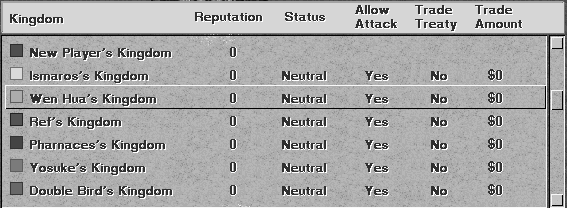
\includegraphics[width=0.85\linewidth]{Idimplomacy} % Original size.
\end{center}

\section{\textsf{Contacting Other Kingdoms}}

\index{diplomacy!contacting other kingdoms}

\textswab{\huge{Y}}ou will be unable to initiate contact with a foreign Kingdom until you have come upon one of their structures or Villages in your explorations.

% May or will see?

For each Kingdom that you have encountered, you may see, on the bottom half of the page, different options as to what kind of messages you can send to them. These differences will arise due to the varying relationships that you may have with these Kingdoms.

\begin{center}
    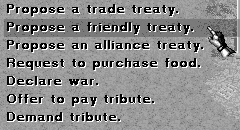
\includegraphics[width=0.4\linewidth]{Idimplomacy_propose} % Original size.
\end{center}

If you wish to send an overture to the selected Kingdom, just \textbf{Click} on the message that you want to send.

Although the message will be dispatched immediately, you will have to wait a while for a reply. Communications in this age are not as fast as you might wish.

\section{\textsf{Replying to Other Kingdoms}}

\index{diplomacy!replying to other kingdoms}

\textswab{\huge{I}}f another Kingdom is contacting you, you will see their message on the bottom left of your screen along with a colored square showing who the message is from.

\begin{center}
    
\includegraphics[width=0.8\linewidth]{Imessage} % Original size.
\end{center}

% Kingdoms screen

To reply to an overture from another Kingdom, \textbf{Click} on the colored square in front of the message. This will take you to the Kingdoms screen where you will see your two options. Just \textbf{Click} on your choice; either Accept or Reject.

These messages will remain on the bottom of your screen for one month. At the end of this time, it is assumed that the message has been rejected, and so it will disappear. This will ensure that all messages will correctly reflect the present world situation.

\section{\textsf{Possible Diplomatic Overtures}}

\index{diplomacy!possible overtures}

\subsection{\textsf{Propose a Trade Treaty}}

\index{diplomacy!trade treaty}
\index{trade!treaty!proposing}

\textswab{\huge{T}}his may only be proposed between Kingdoms that are not already Allied. Allied Kingdoms are automatically bound to Trade with each other.

When Trade Treaties are in effect, Treaty partners are allowed to pick up goods from each other’s Markets.

% Choppy here.

They are also allowed to build their own Markets near their partner’s Villages. If they do this and if they are selling the same goods as are for sale in their partner’s Markets, then the Villagers will buy from their own Markets first and then, if their demand cannot be sated, from the Market of the foreign Treaty partner.

\subsection{\textsf{Propose a Friendly Treaty}}

\index{diplomacy!friendly treaty}
\index{friendly treaty!proposing}

\textswab{\huge{T}}his may only be proposed between Kingdoms whose relations are either Neutral or Tense.

The only binding element of such a Treaty is that the signatory Kingdoms must not attack each other.

\subsection{\textsf{Propose an Alliance Treaty}}

\index{alliance treaty!proposing}
\index{diplomacy!alliance treaty}

\textswab{\huge{T}}his may only be proposed between Kingdoms whose relations are either Neutral or Friendly.

Kingdoms in an Alliance Treaty will automatically be considered to have a Trade Treaty.

An added benefit is that even when the Fog of War is on, Allies will be able to see each others’ units, Villages, and Buildings.

Kingdoms in an Alliance may come to the aid of each other when under attack by enemy Kingdoms or by Fryhtans.

\subsection{\textsf{Request Immediate Military Aid}}

\index{military aid}

\textswab{\huge{T}}his request may be made only to an Allied or a Friendly Kingdom and only if the requesting Kingdom is presently at war with either another Kingdom, with an Independent Village, or with Fryhtans.

If the request is accepted, military forces will be immediately dispatched to the nearest battle in which the requesting Kingdom’s soldiers are taking part.

When the last of the enemy is destroyed, the requested forces will return to their previous positions.

\subsection{\textsf{Request a Trade Embargo}}

\index{trade!embargo}

\textswab{\huge{T}}his request may be made only to Allied or Friendly Kingdoms. You are requesting that they terminate any Trade Treaties that they might have with a certain Kingdom.

% Hyphenated 'non" here.

When you make this request, you will be presented with a list of all Non-Allied Kingdoms. You may not Embargo trade with Allied Kingdoms.

When you \textbf{Click} on the targeted Kingdom, your request will be sent.

\subsection{\textsf{Terminate Our Trade Treaty}}

\index{trade!treaty!terminating}

\textswab{\huge{T}}his may only be proposed to a Kingdom when that Kingdom is not an Ally as Allies are bound to Trade with each other.

\subsection{\textsf{Terminate Our Friendly Treaty}}

\index{friendly treaty!terminating}

\textswab{\huge{T}}his may only be proposed to a Kingdom when relations with that Kingdom are Friendly.

\subsection{\textsf{Terminate Our Alliance Treaty}}

\index{alliance treaty!terminating} 

\textswab{\huge{T}}his may only be proposed to a Kingdom that is an Ally.

\subsection{\textsf{Request a Cease-Fire}}

\index{cease-fire}

\textswab{\huge{T}}his may only be requested by a Kingdom currently at War with another.

\subsection{\textsf{Request a Declaration of War against a Foe}}

\index{declaration of war}

\textswab{\huge{T}}his may only be requested of an Allied Kingdom.

You will be presented with a list of Kingdoms. When you \textbf{Click} on the targeted Kingdom, your message will be sent.

\subsection{\textsf{Request to Purchase Food}}

\index{request to purchase food}

\textswab{\huge{T}}his may only be requested by Kingdoms that are not at War with each other.

The Kingdom making the request will be asked for the monetary amount that it wishes to spend. When the amount is \textbf{Clicked} on, the offer will be sent.

\subsection{\textsf{Declare War}}

\index{declaration of war}
\index{diplomacy!declaration of war}

\textswab{\huge{T}}his may only be Declared by Kingdoms that are not already at war with one another.

If you wish to avoid a great loss to your Reputation, it is a good idea to Declare War \textit{before} you attack.

\subsection{\textsf{Offer to Pay Tribute}}

\index{tribute!offer to pay}

\textswab{\huge{T}}his may be proposed at any time between Kingdoms that are at War or whose relations are Tense or Neutral.

Paying Tribute to another Kingdom will make it more likely that the receiver of the Tribute will look upon future proposals from the Tributary with more good will.

The Kingdom making the offer will be presented with a list of amounts. When the selected amount is \textbf{Clicked} on, the offer will be sent.

\subsection{\textsf{Demand Tribute}}

\index{tribute!demand for}

\textswab{\huge{T}}ribute may be demanded only from a Kingdom that is at War or that has Tense or Neutral relations with the demander.

If Tribute is granted, it is more likely that the demanding Kingdom will work to improve its relations with the Kingdom that pays.

% Accept or comply?

If your Kingdom is on the receiving end of a demand, you will be notified of the demanded amount. If you choose to accept the demand, your money will be transferred to the demanding Kingdom.

If you are making the demand, you will be presented with a list of amounts. When you \textbf{Click} on the desired amount, the demand will be sent.

\subsection{\textsf{Offer to Transfer Technology}}

\index{transferring technology}

\textswab{\huge{T}}echnology may be transferred between Kingdoms only if they are Allied or Friendly.

You will be presented with a list of technologies that you wish to transfer. When you \textbf{Click} on the intended technology, the offer will be sent.

The offer of technology will be rejected if the other Kingdom already possesses it. If they do not possess it, they will certainly and gratefully accept.

\subsection{\textsf{Request Technology}}

\index{requesting technology}

\textswab{\huge{A}} request for technology may be made only to an Allied or a Friendly Kingdom.

If you are requesting a transfer, you will be presented with a list of technologies. When you \textbf{Click} on one, your request will be sent. This process will be much more efficient if you know exactly which technologies other Kingdoms possess. That, among other thing, is what Spies are for.

If another Kingdom is requesting a transfer from you, you will be told which technology it is that they desire. If you accept, they will immediately receive the technology.

\subsection{\textsf{Offer Aid}}

\textswab{\huge{A}}id may be offered to all Kingdoms except for those that are at War with each other.

The offering \index{aid!offering} of Aid will influence future relations by making those who have been offered Aid more friendly towards those who have made the offer.

\subsection{\textsf{Request Aid}}

\index{aid!requesting}

\textswab{\huge{T}}his may only be requested from Kingdoms that are Allied or Friendly.

If you are requesting Aid, you will be presented with a list of amounts. When you \textbf{Click} on the desired amount, your request will be sent.

If another Kingdom is requesting Aid from you, you will be notified of the amount of the request. If you accept, the amount will be immediately transferred.

\subsection{\textsf{Offer to Purchase Throne and Unite Kingdoms}}

\index{purchasing throne}
\index{uniting kingdoms}

\textswab{\huge{W}}ith this request, you may be able to purchase the throne, people, and property of another Kingdom.

It is unlikely that your offer will be considered if your Kingdom suffers from a poor Reputation or if it lacks the funds to make an enticing offer.

If you receive this offer from another Kingdom and accept it, you shall immediately relinquish your entire Kingdom. The money that you receive will be added to your final score.

If you wish to continue to watch, you will see your former King in his new role as a General in the army of the united Kingdom.

\subsection{\textsf{Surrender}}

\index{surrender}

\begin{wrapfigure}{r}{0.6\textwidth}
    \vspace{-20pt}
    \begin{center}
        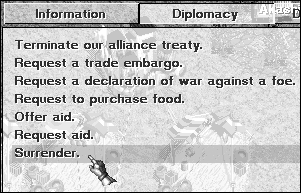
\includegraphics[width=0.6\textwidth]{Idimplomacy_surrender} % Original size.
    \end{center}
    \vspace{-20pt}
\end{wrapfigure}

\textswab{\huge{S}}urrender is always an option for a Kingdom in dire straits. It offers you the option of turning your possessions and people over to a friendly King who may then carry on your fight.

When you \textbf{Click} on the Surrender option, you will be asked if you are sure.

\begin{center}
    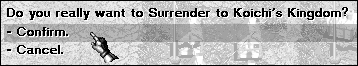
\includegraphics[width=0.7\linewidth]{Isurrender_responce} % Original size.
\end{center}

If you are quite sure, \textbf{Click} on the Confirm line. When you have done so, all of your people and possessions will be put under the control of the selected Kingdom. You may then continue to observe the game if you so wish.

\section{\textsf{Changes in Diplomatic Status}}

\index{changes in diplomatic status}

\subsection{\textsf{From Friendly}}

\textswab{\huge{W}}hen one Kingdom ends a Friendly Treaty with another, their status will change to Neutral.

When one Kingdom attacks or Declares War on another, their status will change to War.

\subsection{\textsf{From Alliance}}

\textswab{\huge{W}}hen one Kingdom withdraws from an Alliance, their relationship to the Allied Kingdoms will change to Neutral.

When one Kingdom in an Alliance attacks or Declares War on another Allied Kingdom, the status of both will change to War.

\subsection{\textsf{From Neutral}}

\textswab{\huge{W}}hen Neutral Kingdoms sign a Friendly Treaty, their status will change to Friendly.

When Neutral Kingdoms sign an Alliance Treaty, their status will change to Alliance.

When Neutral Kingdoms attack or Declare War on each other, their status will change to War.

\subsection{\textsf{From Tense}}

\textswab{\huge{T}}wo Tense Kingdoms who have not fought for three years will change their status to Neutral.

When two Tense Kingdoms sign a Friendly Treaty, their status will change to Friendly.

When two Tense Kingdoms sign an Alliance Treaty, their status will change to Alliance.

When a Tense Kingdom attacks or Declares War on another, their status will change to War.

\subsection{\textsf{From War}}

% in a War relationship = at war.

\textswab{\huge{W}}hen two Kingdoms in a War relationship have not fought for three years, their status will change to Tense.

\section{\textsf{Information}}

% (F1) here.

\textswab{\huge{W}}hen you are in the Kingdoms Report (F1), \textbf{Clicking} on the \textbf{Information Button} will show information on the relationship between the selected Kingdom and your Kingdom.

\section{\textsf{Multiplayer Chat}}

% Index right?

\index{chat, multiplayer}
\index{Mutiplayer!chat}

% Informal. Key here

\textswab{\huge{I}}f you are in a multiplayer game and wish to chat with your human opponents, \textbf{Click} on the \textbf{Chat Button}. This will take you to the chat page. To send a message, \textbf{Click} on the Kingdom that you wish to chat with, type your message, and press Enter. You may send a message to more than one player at a time by \textbf{Clicking} on either the second or third option buttons that you can see on the bottom of the chat screen.

\begin{center}
    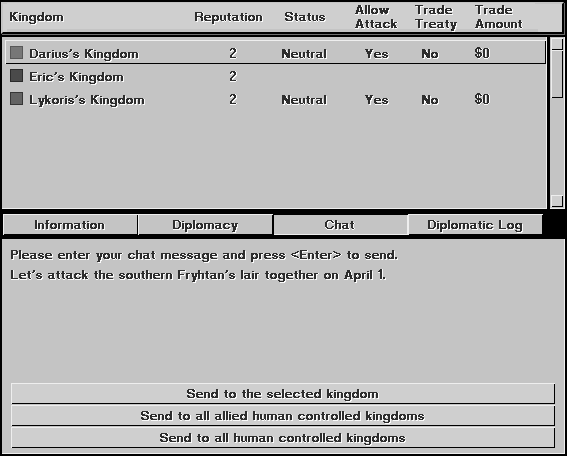
\includegraphics[width=0.85\linewidth]{Imutlichat} % Original size?
\end{center}

To answer a chat message, \textbf {Click} on the colored square in front of it. That will take you to the chat page where you can type your reply. Your reply will then appear on the bottom of the original poster’s screen.

\begin{center}
    
\includegraphics[width=0.85\linewidth]{Imutlichat_message} % Original size.
\end{center}

\section{\textsf{Diplomatic Message Logs}}

\index{diplomatic message logs}

% (F1)

\textswab{\huge{W}}hen you are in the Kingdoms Report (F1), \textbf{Click} on the \textbf{Diplomatic Log Button}. These Diplomatic Logs will show you all of your past Diplomatic correspondence.

If your own Kingdom is selected in the Kingdoms list, the log will display the diplomatic messages that have gone to or from your Kingdom in the recent past.

If another Kingdom is selected in the Kingdoms list, the log will display the diplomatic messages that have traveled between your Kingdom and the selected Kingdom in the recent past.